\section{Electron Transport Chain and Oxidative Phosphorylation}

\begin{objectivebox}
After completing this section, you should be able to:
\begin{itemize}
    \item Describe the location and components of the electron transport chain
    \item Explain the function of each complex (I-IV) and mobile electron carriers
    \item Describe the chemiosmotic theory and proton motive force
    \item Explain ATP synthesis by ATP synthase
    \item Calculate ATP yield from glucose oxidation
    \item Identify inhibitors and uncouplers of oxidative phosphorylation
\end{itemize}
\end{objectivebox}

\subsection{Overview of Oxidative Phosphorylation}

\begin{definition}
\textbf{Oxidative phosphorylation} is the process by which ATP is synthesized using energy released from the transfer of electrons from NADH and FADH$_2$ to oxygen through a series of electron carriers in the inner mitochondrial membrane.
\end{definition}

\textbf{Two coupled processes:}
\begin{enumerate}
    \item \textbf{Electron transport chain (ETC)}: Electrons flow from NADH/FADH$_2$ to O$_2$, releasing energy used to pump H$^+$
    \item \textbf{Chemiosmosis}: H$^+$ flows back through ATP synthase, driving ATP synthesis
\end{enumerate}

\subsection{Mitochondrial Structure}

\begin{center}
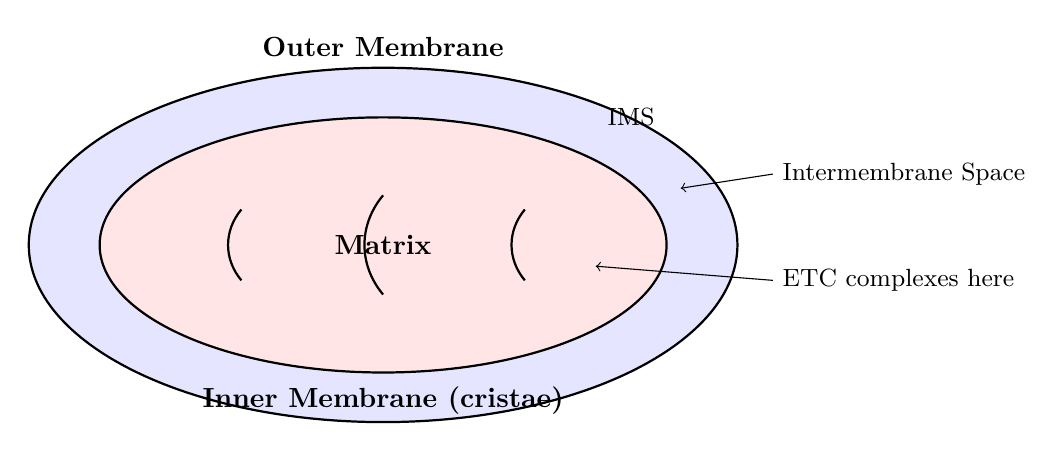
\begin{tikzpicture}[scale=0.9]
    % Outer membrane
    \draw[thick, fill=blue!10] (0,0) ellipse (5cm and 2.5cm);
    \node at (0, 2.8) {\textbf{Outer Membrane}};
    
    % Intermembrane space
    \node at (3.5, 1.8) {\small IMS};
    
    % Inner membrane with cristae
    \draw[thick, fill=red!10] (0,0) ellipse (4cm and 1.8cm);
    \draw[thick] (-2, 0.5) to[bend right=40] (-2, -0.5);
    \draw[thick] (0, 0.7) to[bend right=40] (0, -0.7);
    \draw[thick] (2, 0.5) to[bend right=40] (2, -0.5);
    \node at (0, -2.2) {\textbf{Inner Membrane (cristae)}};
    
    % Matrix
    \node at (0, 0) {\textbf{Matrix}};
    
    % Labels
    \draw[->] (5.5, 1) -- (4.2, 0.8);
    \node[right] at (5.5, 1) {\small Intermembrane Space};
    
    \draw[->] (5.5, -0.5) -- (3, -0.3);
    \node[right] at (5.5, -0.5) {\small ETC complexes here};
\end{tikzpicture}
\end{center}

\textbf{Key locations:}
\begin{itemize}
    \item \textbf{Outer membrane}: Permeable to small molecules (contains porins)
    \item \textbf{Intermembrane space (IMS)}: Site of H$^+$ accumulation; similar composition to cytosol
    \item \textbf{Inner membrane}: Impermeable to most molecules; contains ETC complexes and ATP synthase
    \item \textbf{Matrix}: Contains TCA cycle enzymes, pyruvate dehydrogenase, mtDNA
\end{itemize}

\subsection{Components of the Electron Transport Chain}

\subsubsection{Complex I: NADH-Ubiquinone Oxidoreductase}

\begin{itemize}
    \item \textbf{Also called}: NADH dehydrogenase
    \item \textbf{Prosthetic groups}: FMN, Fe-S clusters
    \item \textbf{Function}: Transfers 2 electrons from NADH to ubiquinone (CoQ)
    \item \textbf{H$^+$ pumped}: 4 H$^+$ per NADH
\end{itemize}

\[
\text{NADH} + \text{H}^+ + \text{Q} \rightarrow \text{NAD}^+ + \text{QH}_2
\]

\subsubsection{Complex II: Succinate-Ubiquinone Oxidoreductase}

\begin{itemize}
    \item \textbf{Also called}: Succinate dehydrogenase (same enzyme as TCA cycle!)
    \item \textbf{Prosthetic groups}: FAD, Fe-S clusters
    \item \textbf{Function}: Transfers electrons from succinate (via FADH$_2$) to ubiquinone
    \item \textbf{H$^+$ pumped}: 0 (no proton pumping!)
\end{itemize}

\[
\text{Succinate} + \text{Q} \rightarrow \text{Fumarate} + \text{QH}_2
\]

\begin{analogy}
Complex II is like a side entrance to the ETC. Electrons from FADH$_2$ enter here, bypassing Complex I. Because they skip the first proton pump, FADH$_2$ produces less ATP than NADH—like getting on a bus at a later stop and paying a reduced fare.
\end{analogy}

\subsubsection{Ubiquinone (Coenzyme Q)}

\begin{itemize}
    \item \textbf{Mobile electron carrier} in the inner membrane
    \item Lipid-soluble (moves freely in membrane)
    \item Accepts electrons from Complex I AND Complex II
    \item Can carry 1 or 2 electrons (semiquinone intermediate)
    \item Delivers electrons to Complex III
\end{itemize}

\subsubsection{Complex III: Ubiquinol-Cytochrome c Oxidoreductase}

\begin{itemize}
    \item \textbf{Also called}: Cytochrome bc$_1$ complex
    \item \textbf{Prosthetic groups}: Heme b, Heme c$_1$, Fe-S cluster (Rieske protein)
    \item \textbf{Function}: Transfers electrons from QH$_2$ to cytochrome c via Q cycle
    \item \textbf{H$^+$ pumped}: 4 H$^+$ per pair of electrons
\end{itemize}

\subsubsection{Cytochrome c}

\begin{itemize}
    \item \textbf{Mobile electron carrier} in intermembrane space
    \item Water-soluble peripheral membrane protein
    \item Contains heme c prosthetic group
    \item Carries only ONE electron at a time
    \item Also plays role in apoptosis when released to cytoplasm
\end{itemize}

\subsubsection{Complex IV: Cytochrome c Oxidase}

\begin{itemize}
    \item \textbf{Function}: Transfers electrons from cytochrome c to O$_2$ (final electron acceptor)
    \item \textbf{Prosthetic groups}: Heme a, Heme a$_3$, Cu$_A$, Cu$_B$
    \item \textbf{H$^+$ pumped}: 2 H$^+$ per pair of electrons
    \item Requires 4 electrons to fully reduce O$_2$ to 2 H$_2$O
\end{itemize}

\[
4 \text{ Cyt c (reduced)} + 4\text{H}^+ + \text{O}_2 \rightarrow 4 \text{ Cyt c (oxidized)} + 2\text{H}_2\text{O}
\]

\begin{tcolorbox}[colback=yellow!10, colframe=yellow!70!black, title=\textbf{Summary: Electron Flow Through ETC}]
\begin{center}
\textbf{NADH pathway:}
\[
\text{NADH} \xrightarrow{\text{Complex I}} \text{Q} \xrightarrow{\text{Complex III}} \text{Cyt c} \xrightarrow{\text{Complex IV}} \text{O}_2
\]

\textbf{FADH$_2$ pathway:}
\[
\text{FADH}_2 \xrightarrow{\text{Complex II}} \text{Q} \xrightarrow{\text{Complex III}} \text{Cyt c} \xrightarrow{\text{Complex IV}} \text{O}_2
\]
\end{center}

\textbf{Total H$^+$ pumped:}
\begin{itemize}
    \item NADH: 4 (CI) + 4 (CIII) + 2 (CIV) = \textbf{10 H$^+$}
    \item FADH$_2$: 0 (CII) + 4 (CIII) + 2 (CIV) = \textbf{6 H$^+$}
\end{itemize}
\end{tcolorbox}

\subsection{Chemiosmotic Theory}

\begin{theorem}
\textbf{Peter Mitchell's Chemiosmotic Theory} (Nobel Prize, 1978):

The energy released during electron transport is used to pump H$^+$ from the matrix to the intermembrane space, creating an \textbf{electrochemical gradient} (proton motive force). The flow of H$^+$ back into the matrix through ATP synthase drives ATP synthesis.
\end{theorem}

\textbf{Proton Motive Force ($\Delta p$) has two components:}

\begin{enumerate}
    \item \textbf{Chemical gradient} ($\Delta$pH): Higher [H$^+$] in IMS than matrix
    \begin{itemize}
        \item IMS: pH $\approx$ 7.0
        \item Matrix: pH $\approx$ 8.0
    \end{itemize}
    
    \item \textbf{Electrical gradient} ($\Delta\psi$): Positive charge in IMS, negative in matrix
    \begin{itemize}
        \item Membrane potential $\approx$ 140 mV (inside negative)
    \end{itemize}
\end{enumerate}

\[
\Delta p = \Delta\psi - \frac{2.3RT}{F}\Delta\text{pH}
\]

\begin{analogy}
The proton motive force is like water behind a dam. The ETC pumps water (H$^+$) uphill to create a reservoir. The pressure of this water (proton motive force) can then be used to turn a
turbine (ATP synthase) and generate electricity (ATP).
\end{analogy}

\subsection{ATP Synthase (Complex V)}

\begin{definition}
\textbf{ATP synthase} (F$_0$F$_1$ ATPase) is a molecular machine that uses the proton motive force to synthesize ATP from ADP and P$_i$.
\end{definition}

\textbf{Structure of ATP Synthase:}

\begin{enumerate}
    \item \textbf{F$_0$ portion} (membrane-embedded):
    \begin{itemize}
        \item Contains the \textbf{c-ring} (proton channel)
        \item Subunit a: provides proton half-channels
        \item c-ring rotation driven by H$^+$ flow
        \item Number of c subunits varies (8-15 depending on species)
    \end{itemize}
    
    \item \textbf{F$_1$ portion} (matrix-facing):
    \begin{itemize}
        \item $\alpha_3\beta_3$ hexamer: catalytic head
        \item $\beta$ subunits contain catalytic sites for ATP synthesis
        \item $\gamma$ subunit: central rotating shaft
        \item $\delta$ and $\epsilon$ subunits: connect F$_0$ to F$_1$
    \end{itemize}
\end{enumerate}

\begin{theorem}
\textbf{Boyer's Binding Change Mechanism} (Nobel Prize, 1997):

The three $\beta$ subunits cycle through three conformational states:
\begin{enumerate}
    \item \textbf{O (Open)}: Low affinity — releases ATP
    \item \textbf{L (Loose)}: Binds ADP + P$_i$ loosely
    \item \textbf{T (Tight)}: High affinity — catalyzes ATP formation
\end{enumerate}

Rotation of the $\gamma$ subunit (driven by H$^+$ flow through F$_0$) causes sequential conformational changes in each $\beta$ subunit.

\textbf{One complete rotation (360°) produces 3 ATP molecules.}
\end{theorem}

\begin{center}
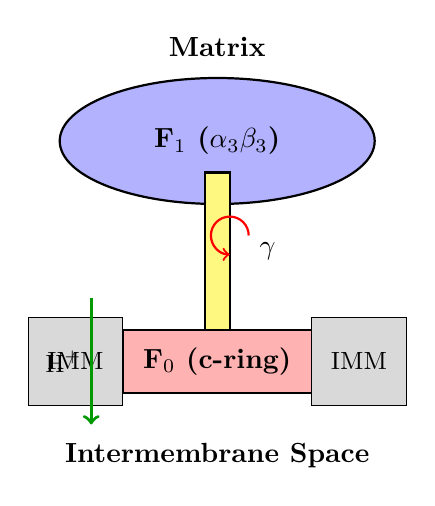
\begin{tikzpicture}[scale=0.8]
    % F1 head
    \draw[fill=blue!30, thick] (0,0) ellipse (2.5cm and 1cm);
    \node at (0,0) {\textbf{F$_1$ ($\alpha_3\beta_3$)}};
    
    % Gamma shaft
    \draw[fill=yellow!50, thick] (-0.2,-0.5) rectangle (0.2,-3);
    \node at (0.8,-1.75) {$\gamma$};
    
    % F0 portion
    \draw[fill=red!30, thick] (-1.5,-3) rectangle (1.5,-4);
    \node at (0,-3.5) {\textbf{F$_0$ (c-ring)}};
    
    % Membrane
    \draw[fill=gray!30] (-3,-2.8) rectangle (-1.5,-4.2);
    \draw[fill=gray!30] (1.5,-2.8) rectangle (3,-4.2);
    \node at (-2.25,-3.5) {\small IMM};
    \node at (2.25,-3.5) {\small IMM};
    
    % Proton flow
    \draw[->, very thick, green!60!black] (-2,-2.5) -- (-2,-4.5);
    \node[left] at (-2,-3.5) {\small H$^+$};
    
    % Labels
    \node at (0,1.5) {\textbf{Matrix}};
    \node at (0,-5) {\textbf{Intermembrane Space}};
    
    % Rotation arrow
    \draw[->, thick, red] (0.5,-1.5) arc (0:270:0.3);
\end{tikzpicture}
\end{center}

\subsection{ATP Yield from Complete Glucose Oxidation}

\begin{center}
\begin{tcolorbox}[colback=green!5, colframe=green!70!black, title=\textbf{Complete ATP Accounting per Glucose}]
\begin{tabular}{lcccc}
\toprule
\textbf{Stage} & \textbf{ATP} & \textbf{NADH} & \textbf{FADH$_2$} & \textbf{ATP Equivalent} \\
\midrule
Glycolysis & 2 & 2 & — & 2 \\
Pyruvate $\rightarrow$ Acetyl-CoA & — & 2 & — & — \\
TCA Cycle (×2) & 2 (GTP) & 6 & 2 & 2 \\
\midrule
\textbf{Subtotal} & 4 & 10 & 2 & 4 \\
\midrule
\multicolumn{5}{l}{\textbf{Oxidative Phosphorylation:}} \\
10 NADH × 2.5 ATP & & & & 25 \\
2 FADH$_2$ × 1.5 ATP & & & & 3 \\
\midrule
\textbf{TOTAL} & & & & \textbf{30-32 ATP} \\
\bottomrule
\end{tabular}

\vspace{0.3cm}
\textbf{Note:} The range (30-32) depends on which shuttle transports cytosolic NADH:
\begin{itemize}
    \item Malate-aspartate shuttle: 2.5 ATP per NADH (total = 32)
    \item Glycerol-3-phosphate shuttle: 1.5 ATP per NADH (total = 30)
\end{itemize}
\end{tcolorbox}
\end{center}

\subsection{Shuttle Systems for Cytosolic NADH}

The inner mitochondrial membrane is impermeable to NADH. Two shuttle systems transfer reducing equivalents from cytosolic NADH into the mitochondrial matrix:

\subsubsection{Malate-Aspartate Shuttle}

\begin{itemize}
    \item Predominant in \textbf{liver, heart, and kidney}
    \item Transfers electrons to mitochondrial NAD$^+$
    \item Produces \textbf{2.5 ATP per cytosolic NADH}
    \item Reversible; can work in either direction
\end{itemize}

\textbf{Mechanism:}
\begin{enumerate}
    \item Cytosolic OAA + NADH $\rightarrow$ Malate + NAD$^+$ (cytosolic malate DH)
    \item Malate enters matrix via malate-$\alpha$KG antiporter
    \item Matrix malate + NAD$^+$ $\rightarrow$ OAA + NADH (mitochondrial malate DH)
    \item OAA converted to aspartate (transamination)
    \item Aspartate exits via glutamate-aspartate antiporter
    \item Aspartate converted back to OAA in cytosol
\end{enumerate}

\subsubsection{Glycerol-3-Phosphate Shuttle}

\begin{itemize}
    \item Predominant in \textbf{brain and skeletal muscle}
    \item Transfers electrons to FAD (via mitochondrial G3P DH)
    \item Produces \textbf{1.5 ATP per cytosolic NADH}
    \item Irreversible; simpler but less efficient
\end{itemize}

\textbf{Mechanism:}
\begin{enumerate}
    \item DHAP + NADH $\rightarrow$ Glycerol-3-P + NAD$^+$ (cytosolic G3P DH)
    \item Glycerol-3-P oxidized by mitochondrial G3P DH (FAD-linked)
    \item FADH$_2$ transfers electrons directly to CoQ
    \item DHAP regenerated and returns to cytosol
\end{enumerate}

\subsection{Inhibitors of Oxidative Phosphorylation}

\begin{center}
\begin{tabular}{llp{6cm}}
\toprule
\textbf{Target} & \textbf{Inhibitor} & \textbf{Effect} \\
\midrule
Complex I & Rotenone, Amytal, MPP$^+$ & Blocks NADH oxidation \\
Complex II & Malonate & Competitive inhibitor (succinate analog) \\
Complex III & Antimycin A & Blocks cytochrome b$_{566}$ \\
Complex IV & CN$^-$, CO, H$_2$S, Azide & Binds to Fe$^{3+}$ in cytochrome a$_3$ \\
ATP Synthase & Oligomycin & Blocks F$_0$ proton channel \\
\bottomrule
\end{tabular}
\end{center}

\begin{example}
\textbf{Cyanide Poisoning:}

Cyanide (CN$^-$) binds tightly to Fe$^{3+}$ in cytochrome c oxidase (Complex IV), preventing electron transfer to O$_2$.

\textbf{Consequences:}
\begin{itemize}
    \item ETC stops completely
    \item No proton gradient formed
    \item No ATP synthesis via oxidative phosphorylation
    \item Cells must rely on glycolysis alone (insufficient for high-energy tissues)
    \item Brain and heart fail rapidly
\end{itemize}

\textbf{Treatment:} Nitrites (convert Hb to MetHb, which binds CN$^-$) followed by thiosulfate (converts CN$^-$ to thiocyanate for excretion)
\end{example}

\subsection{Uncouplers of Oxidative Phosphorylation}

\begin{definition}
\textbf{Uncouplers} are lipid-soluble weak acids that carry H$^+$ across the inner mitochondrial membrane, dissipating the proton gradient without ATP synthesis. Electron transport continues (even accelerates), but energy is released as \textbf{heat}.
\end{definition}

\textbf{Examples of Uncouplers:}
\begin{itemize}
    \item \textbf{2,4-Dinitrophenol (DNP)}: Historical diet pill (dangerous!)
    \item \textbf{FCCP/CCCP}: Laboratory uncouplers
    \item \textbf{Aspirin} (high doses): Weak uncoupling effect
    \item \textbf{Thermogenin (UCP1)}: Natural uncoupler in brown fat
\end{itemize}

\begin{theorem}
\textbf{Brown Adipose Tissue and Thermogenesis:}

Brown fat contains \textbf{uncoupling protein 1 (UCP1/thermogenin)}, which allows H$^+$ to flow back into the matrix without passing through ATP synthase.

\textbf{Function:} Generate heat for:
\begin{itemize}
    \item Thermoregulation in newborns
    \item Non-shivering thermogenesis in cold exposure
    \item Hibernating animals
\end{itemize}

\textbf{Regulation:} Activated by norepinephrine (sympathetic nervous system) and free fatty acids
\end{theorem}

\begin{analogy}
Uncouplers are like holes in a dam. The water (H$^+$) flows through the holes instead of the turbine (ATP synthase). The potential energy is wasted as the water crashes down (heat) rather than doing useful work (ATP).
\end{analogy}

\subsection{Regulation of Oxidative Phosphorylation}

\begin{theorem}
\textbf{Respiratory Control:}

The rate of oxidative phosphorylation is tightly coupled to ATP demand through:

\begin{enumerate}
    \item \textbf{Availability of ADP}: Primary regulator
    \begin{itemize}
        \item High ADP $\rightarrow$ stimulates ATP synthase $\rightarrow$ increases ETC rate
        \item Low ADP $\rightarrow$ ATP synthase slows $\rightarrow$ ETC backs up
    \end{itemize}
    
    \item \textbf{Availability of substrates}: NADH, FADH$_2$, O$_2$
    
    \item \textbf{ATP/ADP ratio}: Reflects cellular energy status
\end{enumerate}
\end{theorem}

\textbf{Respiratory States:}
\begin{itemize}
    \item \textbf{State 3}: Active respiration (ADP present, substrate present)
    \item \textbf{State 4}: Resting respiration (ADP depleted, substrate present)
    \item \textbf{Respiratory Control Ratio (RCR)}: State 3 / State 4 rate
    \begin{itemize}
        \item Normal: 5-10 (tightly coupled)
        \item Uncoupled: approaches 1
    \end{itemize}
\end{itemize}

%%%%%%%%%%%%%%%%%%%%%%%%%%%%%%%%%%%%%%%%%%%%%%%%%%%%%%%%%%%%%%%
